% Bar Chart - EE-Bruttostromerzeugung 2019

\begin{figure}[H]
	\centering
	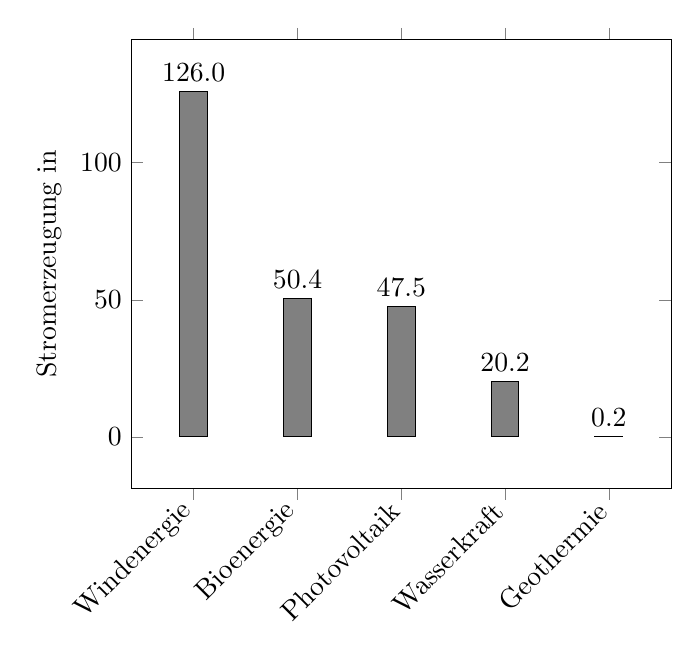
\begin{tikzpicture}
		\begin{axis}[
		ybar,
		enlargelimits=0.15,											% äüßerste bar plots nicht am Limit der x-Achse
		ylabel={Stromerzeugung in \SI{}{\twh}},
		symbolic x coords={Windenergie,
			Bioenergie,
			Photovoltaik,
			Wasserkraft,
			Geothermie 
		},
		xtick=data,
		nodes near coords,											% Zahlen auf den bar plots
		nodes near coords align={vertical},
		nodes near coords style={/pgf/number format/.cd,fixed,fixed zerofill,precision=1},
		x tick label style={rotate=45,anchor=east},
		]
		\addplot[black,fill=black!50!white] coordinates {
			(Windenergie,126.0) (Bioenergie,50.4) (Photovoltaik,47.5) (Wasserkraft,20.2) (Geothermie,0.2)
		};
		\end{axis}
	\end{tikzpicture}
	\caption{Verteilung der Bruttostromerzeugung aus erneuerbaren Energien nach Erzeugungsart im Jahr 2019 \parencite{BWE2020}; \textit{Eigene Darstellung}}
	\label{fig:ee-gen_total}
\end{figure}